\documentclass[journal]{IEEEtran}
\usepackage[T1]{fontenc}
\usepackage{amsmath,amsfonts}
\usepackage{algorithmic}
\usepackage{algorithm}
\usepackage{array}
\usepackage[caption=false,font=normalsize,labelfont=sf,textfont=sf]{subfig}
\usepackage{textcomp}
\usepackage{stfloats}
\usepackage{url}
\usepackage{verbatim}
\usepackage{graphicx}
\usepackage{cite}
\usepackage{multirow,array}
\usepackage{amssymb}
\usepackage{cite}
\makeatletter
\newcommand{\rmnum}[1]{\romannumeral #1} % 小写罗马数字
\newcommand{\Rmnum}[1]{\expandafter\@slowromancap\romannumeral #1@} % 大写罗马数字
\makeatother
\usepackage{float}
\usepackage{placeins}
\hyphenation{op-tical net-works semi-conduc-tor IEEE-Xplore}
% updated with editorial comments 8/9/2021

\begin{document}

\title{Consensus-Guided Pseudo-Labeling via Heterogeneous Speech Ensembles for Robust Unsupervised Speaker Verification}

\author{Heng Wu, Yishuang Li, Hongchen Pan, Lin Li~\IEEEmembership{Member,~IEEE}, and Qingyang Hong~\IEEEmembership{Member,~IEEE}
        % <-this % stops a space
% \thanks{This paper was produced by the IEEE Publication Technology Group. They are in Piscataway, NJ.}% <-this % stops a space
% \thanks{Manuscript received April 19, 2021; revised August 16, 2021.}
}

% The paper headers
\markboth{IEEE TRANSACTIONS ON AUDIO, SPEECH, AND LANGUAGE PROCESSING,,~Vol.~1, No.~1, January ~2025}%
{Shell \MakeLowercase{\textit{et al.}}: A Sample Article Using IEEEtran.cls for IEEE Journals}

%\IEEEpubid{0000--0000/00\$00.00~\copyright~2021 IEEE}
% Remember, if you use this you must call \IEEEpubidadjcol in the second
% column for its text to clear the IEEEpubid mark.

\maketitle

\begin{abstract}
Unsupervised speaker verification aims to learn speaker-discriminative representations from unlabeled speech, but iterative pseudo-label training is vulnerable to early clustering errors. Pseudo-label ambiguity and speaker-cluster over-segmentation may introduce unreliable supervision and propagate errors across refinement iterations.
In this paper, we propose a consensus-guided pseudo-labeling (CGPL) framework for robust unsupervised speaker verification. From an ensemble-learning perspective, two heterogeneous speech pre-trained models serve as complementary ensemble members and produce two clustering partitions. After cluster-label alignment, cross-model assignment agreement provides an observable consensus signal for selecting pseudo-labeled samples, followed by pseudo-label merging to reduce over-segmentation among highly similar speaker clusters. For model training, selected pseudo-labels are optimized with dynamic label-noise-aware supervision, which uses model predictions as confidence-weighted auxiliary targets rather than replacing the original pseudo-labels. Samples without cross-model consensus are further exploited by self-supervised contrastive learning with hard negative mining.
Experiments on VoxCeleb2 show that the proposed
framework achieves EERs of 1.01\%, 1.36\%, and 2.53\% on Vox1-O,
Vox1-E, and Vox1-H after three refinement iterations, respectively.
Compared with representative state-of-the-art unsupervised speaker verification systems, the proposed framework
achieves lower EERs with fewer
refinement iterations. Notably, the proposed unsupervised
system obtains performance comparable to the fully supervised system
with the same speaker encoder backbone, without using speaker identity
annotations during training.
\end{abstract}

\begin{IEEEkeywords}
Unsupervised speaker verification, ensemble learning, pseudo-label, label-noise-aware supervision, hard negative mining.
\end{IEEEkeywords}

\section{Introduction}

\IEEEPARstart{S}{peaker} verification determines whether a test
utterance belongs to a claimed speaker and is widely used in
speech-based authentication. Deep neural network-based systems
[1]--[5] have substantially improved speaker verification performance
over traditional approaches [6], [7]. These advances, however, largely
depend on large-scale speaker-labeled corpora. Although speech data can
be collected at scale, reliable speaker identity annotations are often
unavailable or require costly manual labeling. This gap between the
availability of speech data and speaker identity labels has motivated
the development of unsupervised speaker verification methods, which aim
to learn speaker-discriminative representations without manual
annotations.

Existing unsupervised speaker verification studies mainly follow two
research directions. The first direction learns speaker representations
through self-supervised objectives. Contrastive learning methods
inspired by SimCLR [8] and MoCo [9] construct positive and negative
speech pairs to learn speaker-discriminative representations without
manual labels [10]--[14]. Self-distillation methods further improve
representation stability by enforcing consistency across different
augmented views while avoiding explicit negative-pair construction
[22]--[30]. The second direction adopts iterative pseudo-label-based
training, where speaker embeddings are clustered to generate
pseudo-labels and the resulting speaker encoder is refined using these
pseudo-labels [15]--[20]. By introducing speaker-level supervision from
unlabeled data, these methods have narrowed the gap between unsupervised
and supervised speaker verification systems. However, their performance
remains highly dependent on the quality of pseudo-label supervision.

Despite recent progress, iterative unsupervised speaker verification is
still challenged by unreliable pseudo-label generation and utilization.
Clustering-based pseudo-labels inevitably contain incorrect assignments
because some samples have ambiguous pseudo-label assignments under imperfect speaker representations.
Moreover, utterances from the same speaker may be divided into multiple
pseudo-label classes, resulting in speaker-cluster over-segmentation.
When these imperfect pseudo-labels are directly used for model
optimization, the introduced errors may be propagated and amplified
during subsequent refinement iterations. Therefore, improving the
quality of pseudo-label supervision and reducing the influence of
residual label noise are critical for achieving robust unsupervised
speaker verification.

Previous studies have attempted to address pseudo-label-related
challenges from different perspectives. Speech self-supervised
pre-trained models, such as wav2vec 2.0, HuBERT, UniSpeech-SAT, and
WavLM [31]--[35], provide transferable representations and have been
shown to improve first-round pseudo-label generation [36].
Noise-resistant learning methods mitigate the influence of noisy
supervision through regularized objectives, reliability-aware
optimization, classifier adjustment, sample selection, or iterative
label refinement [37]--[42]. Other approaches refine clustering results
by filtering samples with low assignment confidence, pruning unreliable classes, or
selecting samples using probabilistic criteria [36], [41], [42].
Although these methods improve representation learning, pseudo-label
generation, or noisy-label optimization, they usually focus on
individual stages of the learning process. In particular, reliable
pseudo-label construction, residual noise mitigation, and effective
utilization of samples with different reliability levels are rarely
considered within a unified framework. As a result, samples without cross-model consensus
are often discarded, while the remaining pseudo-labels may still
contain residual errors.

To address these limitations, we propose a Consensus-Guided
Pseudo-Labeling framework, termed CGPL, for robust unsupervised
speaker verification. CGPL formulates initial pseudo-label generation as
heterogeneous ensemble inference: two speech pre-trained models act as
complementary ensemble members, and their aligned clustering assignments
provide an explicit consensus signal. The framework improves the
reliability of pseudo-label supervision while utilizing both
consensus-selected and cross-view-disagreement samples in a unified
noise-robust training pipeline. Specifically, CGPL uses cross-model
clustering agreement to identify reliable pseudo-labels, introduces
pseudo-label merging to alleviate speaker-cluster over-segmentation,
and further applies noise-robust optimization strategies to handle
residual pseudo-label errors and exploit cross-view-disagreement samples. The main
contributions of this work are summarized as follows:

\begin{itemize}
    \item We formulate initial pseudo-label generation from a heterogeneous
    ensemble-learning perspective and propose a consensus-guided
    pseudo-labeling framework for robust unsupervised speaker verification.
    Cross-model assignment agreement is used as an explicit and operational
    reliability criterion for pseudo-label selection.

    \item We develop a reliability-aware pseudo-label construction strategy
    that combines consensus-guided sample selection and pseudo-label merging
    to improve pseudo-label consistency while alleviating speaker-cluster
    over-segmentation.

    \item We propose a noise-robust training strategy for utilizing unlabeled
    samples with different reliability levels. Consensus-selected samples are optimized
    with dynamic label-noise-aware supervision, while cross-view-disagreement samples are
    further exploited through self-supervised contrastive learning with hard
    negative mining.

    \item Extensive experiments on VoxCeleb benchmarks demonstrate that the
    proposed framework improves pseudo-label quality and speaker verification
    performance, achieving competitive results with fewer refinement
    iterations compared with representative unsupervised speaker verification
    methods.
\end{itemize}


The remainder of this paper is organized as follows.
Section~II reviews related work on unsupervised speaker verification and noise-resistant learning.
Section~III formulates the problem of reliability-aware unsupervised speaker verification and provides an overview of the proposed CGPL framework.
Section~IV presents the proposed consensus-guided pseudo-label construction procedure, including cross-model agreement-based sample selection and pseudo-label merging.
Section~V describes the noise-robust utilization of consensus-selected and cross-view-disagreement samples, where selected pseudo-labeled samples are optimized with dynamic label-noise-aware supervision and the remaining samples are exploited through self-supervised contrastive learning.
Section~VI reports the experimental results and analyses, including the main comparison results, pseudo-label quality analysis, ablation studies, iterative refinement behavior, sensitivity analysis, and complexity analysis.
Finally, Section~VII concludes this paper.

\section{Related Work}

\subsection{Contrastive Learning for Speaker Representation}

Contrastive learning has been widely adopted for unsupervised
speaker representation learning because it can exploit unlabeled
speech through pairwise similarity constraints. Inspired by
frameworks such as SimCLR~[8] and MoCo~[9], previous studies
[10]--[14] construct positive pairs from augmented views or segments
of the same utterance and generally treat samples from different
utterances as negative pairs. The resulting objectives encourage
representations from the same utterance to remain close while
separating those from different utterances.

The effectiveness of contrastive learning, however, depends on the
validity of the negative-pair assumption. In large-scale unlabeled
speech corpora, different utterances may originate from the same
speaker and can therefore be incorrectly treated as negatives. Such
false negatives introduce repulsive constraints between same-speaker
samples and may degrade the learned representation~[21]. Although
existing studies improve contrastive speaker learning through data
augmentation, margin-based objectives, positive-pair construction,
and sample selection~[10]--[14], contrastive learning alone does not
provide explicit pseudo-label supervision and cannot directly address
pseudo-label noise in iterative clustering-based systems.

\subsection{Self-Distillation for Speaker Representation Learning}

Self-distillation provides an alternative self-supervised paradigm
that avoids explicit negative-pair construction. Methods based on
teacher--student architectures enforce prediction consistency across
multiple augmented views and have been applied to unsupervised
speaker representation learning~[22]--[26]. By removing manually
defined negative pairs, these methods reduce the direct influence of
false-negative sampling and improve representation stability.

Self-distillation has also been incorporated into iterative
unsupervised speaker verification frameworks~[27]--[30]. In these
systems, the learned representations are clustered to generate
pseudo-labels for subsequent model refinement. Although
self-distillation improves the robustness of the underlying
representations, it does not directly guarantee reliable clustering
assignments. Ambiguous samples may still receive incorrect
pseudo-labels, and utterances from the same speaker may be split into
multiple pseudo-label classes. Therefore, additional mechanisms are
needed to improve pseudo-label reliability during iterative training.

\subsection{Pre-Trained Models for Unsupervised Speaker Verification}

Speech self-supervised pre-trained models have become important
feature extractors for unsupervised speaker verification. Models such
as wav2vec 2.0~[32], HuBERT~[33], UniSpeech-SAT~[34], and
WavLM~[35] learn transferable representations from large-scale
unlabeled speech and encode acoustic, phonetic, and speaker-related
information that can support downstream speech tasks~[44].

Previous studies~[36], [49] have shown that features extracted from
speech pre-trained models can improve clustering initialization and
unsupervised speaker verification performance. In particular, these
representations provide informative embeddings during the early stage
of iterative pseudo-label training and can be combined with
downstream speaker encoders to incorporate both pre-trained and
task-specific information.

Nevertheless, improved representations do not necessarily lead to
fully reliable pseudo-labels. Early clustering results may still
contain samples with ambiguous pseudo-label assignments, and utterances from the same speaker
may still be divided into multiple pseudo-label classes. Moreover,
speech pre-trained models trained with different objectives may
produce non-identical clustering partitions and error patterns. This
diversity makes heterogeneous pre-trained models suitable ensemble
members: consistent decisions provide a stronger reliability cue than
the output of either individual model.

\subsection{Ensemble Learning and Cross-Model Consensus}

Ensemble learning combines predictions from multiple learners to obtain
more reliable decisions than those produced by an individual learner
[66], [67]. Its effectiveness depends not only on the competence of the
members but also on diversity among their error patterns. In unsupervised
learning, where reference labels are unavailable, agreement among
heterogeneous members can serve as an observable indicator of decision
stability, while disagreement indicates that the inferred assignment is
model-dependent.

Most ensemble methods aggregate class posteriors or discrete predictions
defined in a shared label space. Clustering ensembles are more challenging
because cluster indices are permutation-invariant and independently
generated partitions may contain different numbers of clusters. Therefore,
cross-model agreement cannot be evaluated until the partitions have been
aligned. CGPL addresses this issue by aligning two heterogeneous PTM-based
partitions and using sample-level assignment agreement as an operational
consensus criterion. The method does not assume that agreement proves label
correctness; rather, it uses agreement to identify pseudo-labels that are
stable across two independently learned representation spaces.

\subsection{Iterative Frameworks for Unsupervised Speaker Verification}

Iterative optimization has been widely used to reduce the performance
gap between unsupervised and supervised speaker verification
systems~[15]--[20]. A typical framework alternates between two
stages. First, speaker embeddings are extracted from unlabeled speech
and clustered to generate pseudo-labels. Second, the pseudo-labels
are used to train or refine a speaker encoder. The updated encoder
then produces new embeddings for the next round of clustering and
model optimization.

This iterative procedure enables speaker representations and
pseudo-labels to improve jointly. Its effectiveness, however, is
sensitive to the quality of the initial clustering results. Incorrect
assignments generated in early iterations may be reinforced in later
rounds, while speaker-cluster over-segmentation can provide
inconsistent supervision for utterances from the same speaker.
Consequently, improvements in representation learning alone may be
insufficient when the pseudo-label supervision remains unreliable.

CGPL follows the iterative unsupervised speaker verification setting
but focuses on pseudo-label reliability and sample utilization.
Instead of treating pseudo-label construction and model optimization
as independent stages, CGPL jointly considers reliable pseudo-label
selection, speaker-cluster over-segmentation, residual label noise,
and the utilization of cross-view-disagreement samples within a unified iterative
framework.


\begin{figure*}[!t]
\centering
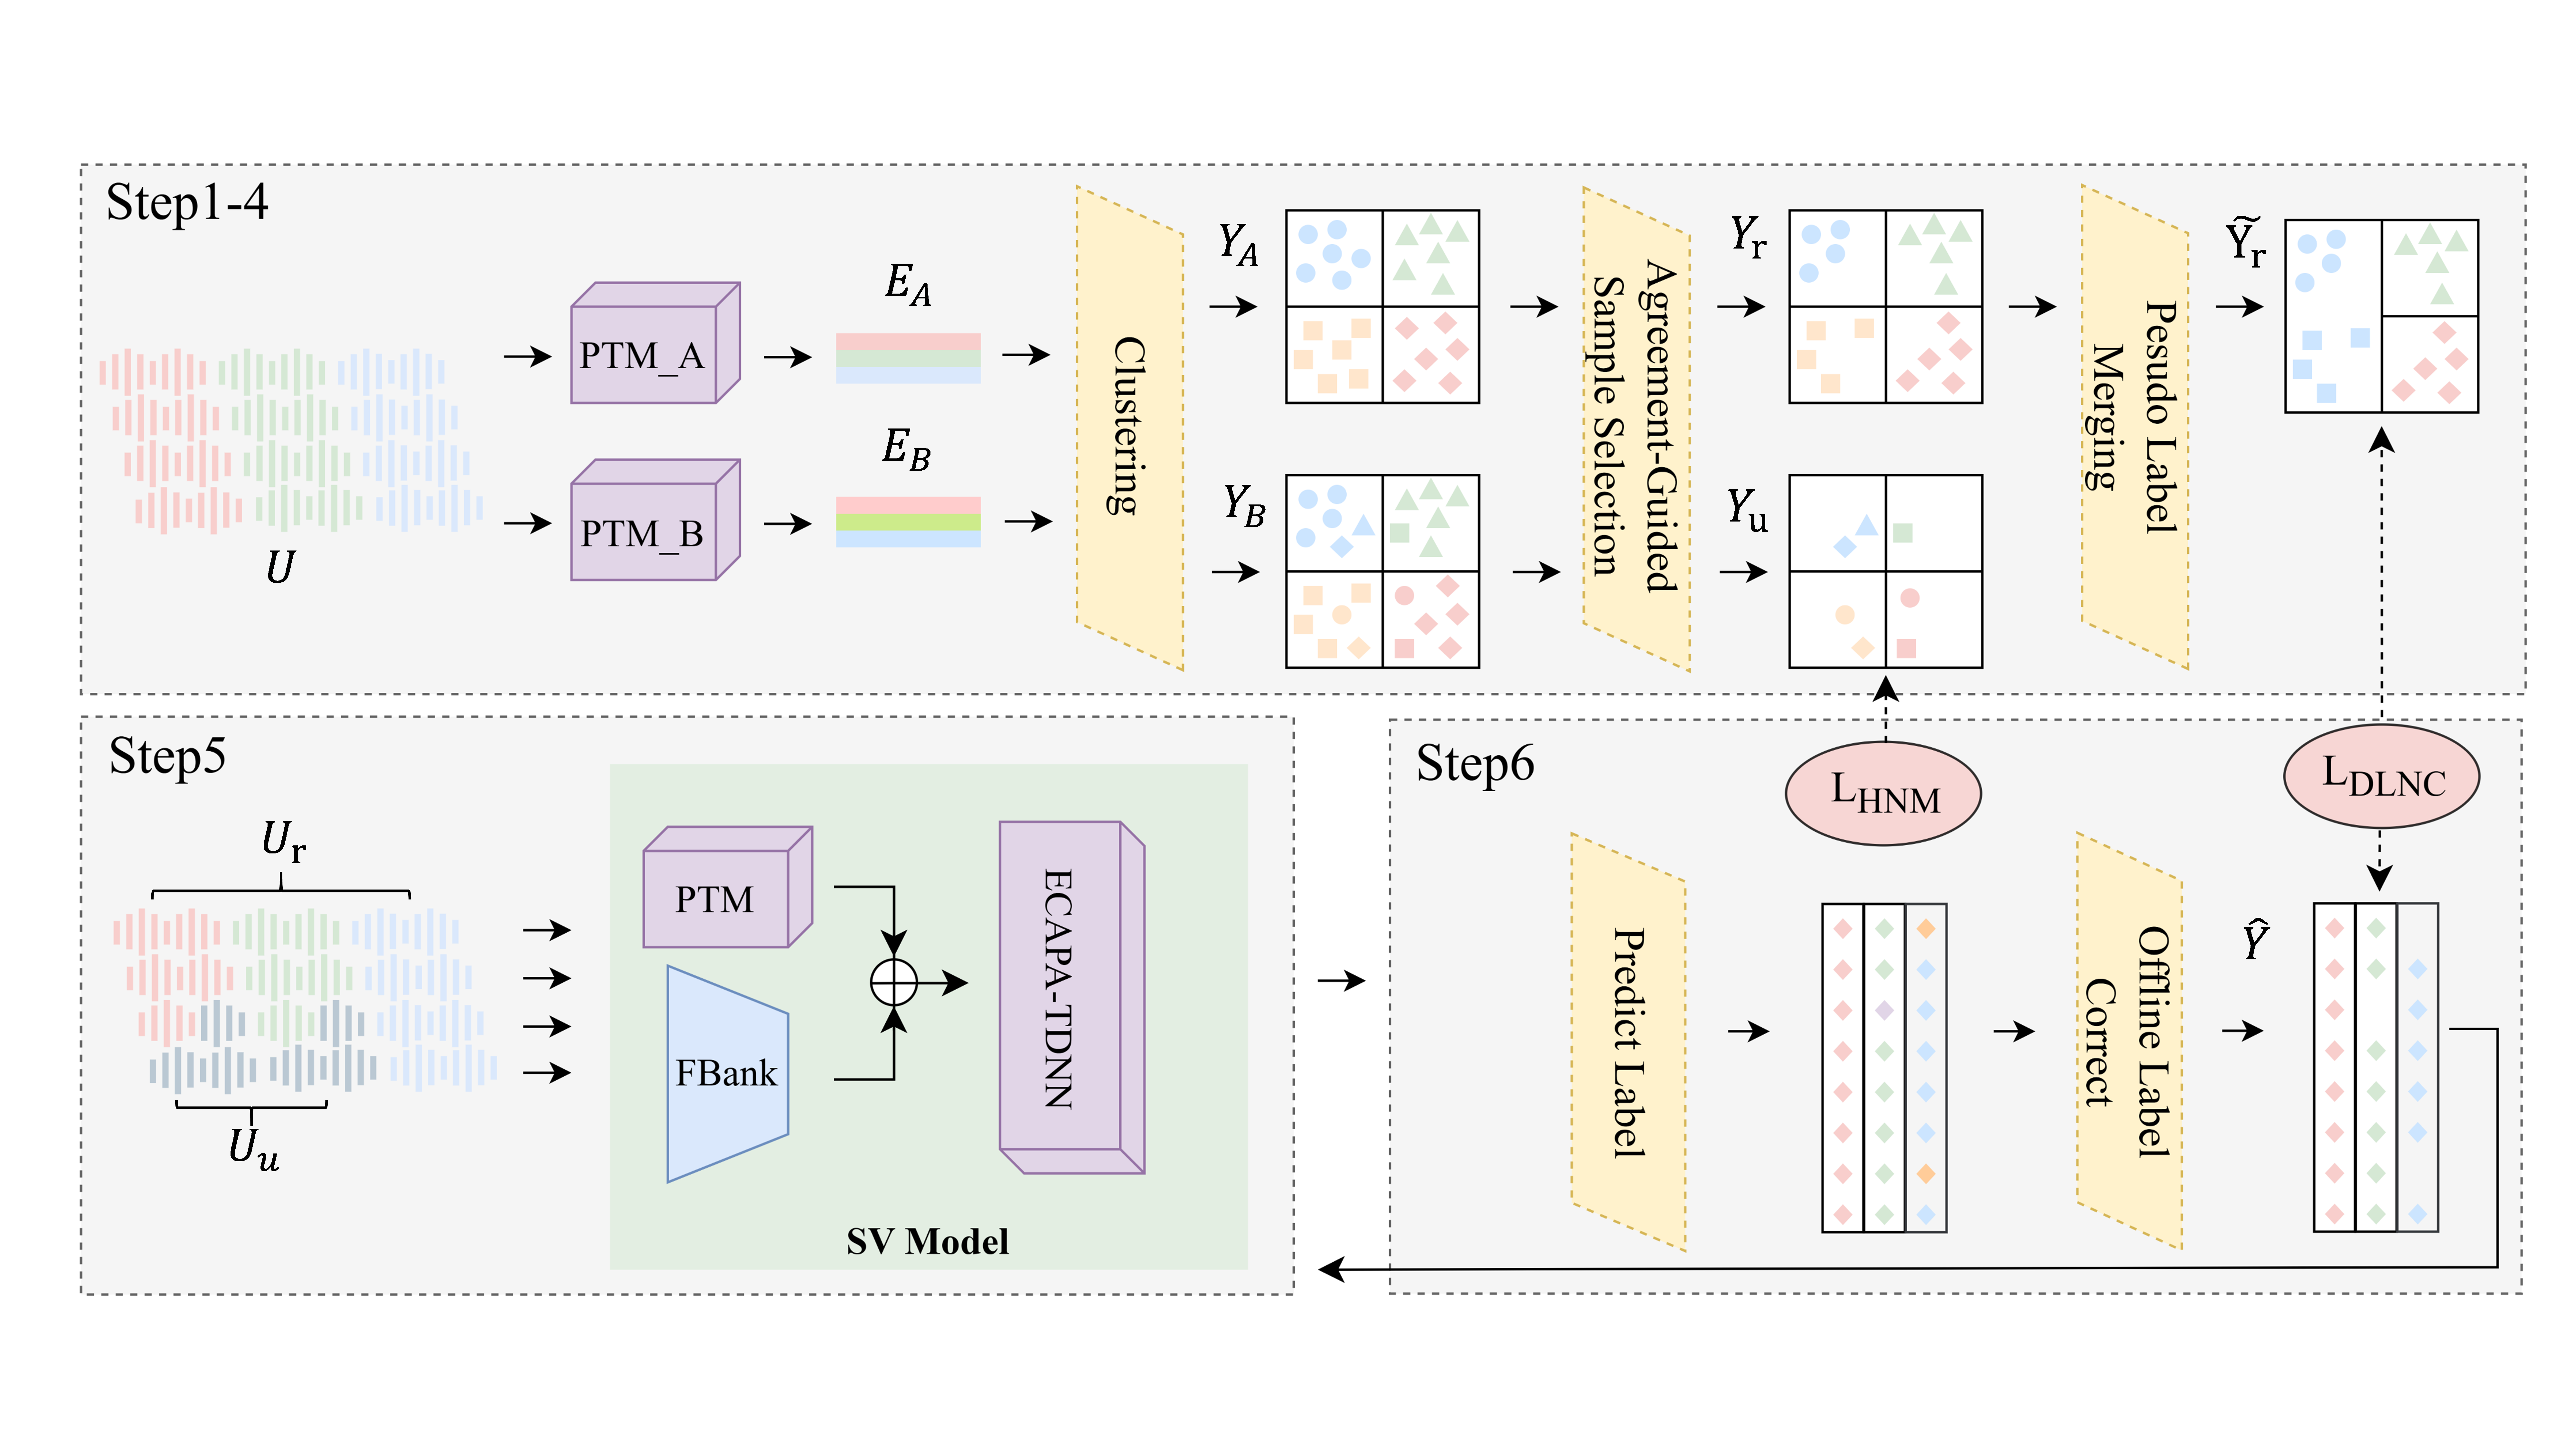
\includegraphics[width=7in]{farme-v3.png}
\caption{{The overall architecture of the proposed CGPL framework.
Steps 1--4 perform consensus-guided reliable pseudo-label construction using two speech pre-trained models, including cluster-label alignment, consensus-based reliable sample selection, and pseudo-label merging.
Steps 5--6 conduct noise-robust utilization of consensus-selected and cross-view-disagreement samples through dynamic label-noise-aware supervision and hard-negative-based contrastive learning.
 }}
\label{fig:frame}
\end{figure*}
\section{Problem Formulation and Framework Overview}

\subsection{Problem Formulation}

Let ${U}=\{x_i\}_{i=1}^{N}$ denote an unlabeled speech corpus, where no speaker identity annotation is available during training. The goal of unsupervised speaker verification is to learn a speaker encoder $f_{\theta}(\cdot)$ that maps an utterance $x_i$ into a speaker-discriminative embedding
\begin{equation}
z_i=f_{\theta}(x_i).
\end{equation}

Since ground-truth speaker labels are unavailable, iterative unsupervised systems usually construct a pseudo-label set
\begin{equation}
\mathcal{Y}=\{y_i\}_{i=1}^{N}
\end{equation}
through clustering and use it as supervision for training $f_{\theta}(\cdot)$.

However, pseudo-labels generated by clustering are not uniformly reliable.
We distinguish two error modes. The first is \emph{assignment noise}: the
pseudo-label assigned to an utterance may not correspond to its latent
speaker identity. The second is \emph{speaker-cluster over-segmentation}:
utterances from one speaker may be distributed across multiple pseudo-label
classes. Once such pseudo-labels are used as hard supervision, their errors
can be reinforced in subsequent refinement iterations.

We use \emph{pseudo-label uncertainty} to describe uncertainty in the
assigned pseudo-label, rather than an intrinsic property of the speech
sample. Because ground-truth labels are unavailable, this uncertainty cannot
be observed directly. Instead, CGPL uses cross-model assignment stability as
an operational proxy. After aligning two clustering partitions, a sample is
defined as \emph{cross-view consistent} if both ensemble members assign it to
the same aligned cluster, and \emph{cross-view discrepant} otherwise. Thus,
discrepancy indicates a model-dependent pseudo-label assignment, but does not
imply that the sample itself is inherently uncertain or that its pseudo-label
is necessarily incorrect.

Based on these definitions, we decompose the learning problem into two
reliability-aware subproblems: constructing a pseudo-label subset supported
by ensemble consensus and robustly utilizing samples with and without such
support.

Specifically, we consider the following two subproblems:

\begin{enumerate}
    \item \textbf{Reliable pseudo-label construction}, which aims to identify a reliable subset
    \begin{equation}
    {U}_{r}\subseteq{U},
    \end{equation}
    whose pseudo-labels are more likely to preserve speaker consistency.

    \item \textbf{Noise-robust sample utilization}, which aims to optimize the speaker encoder by assigning different learning objectives to the consensus-selected subset ${U}_{r}$ and the cross-view-disagreement subset
    \begin{equation}
    {U}_{d}={U}\setminus{U}_{r}.
    \end{equation}
\end{enumerate}

\subsection{Framework Overview}

The proposed framework follows the above decomposition and consists of two sequential stages built on a standard iterative pseudo-label training pipeline.

In the first stage, a heterogeneous ensemble of two speech pre-trained models independently produces two clustering partitions. Since cluster indices are permutation-invariant, the partitions are aligned before their decisions are compared. Samples with identical aligned assignments form the consensus-selected subset. A pseudo-label merging strategy then merges highly similar clusters to alleviate speaker-cluster over-segmentation.

In the second stage, the selected reliable samples are used for pseudo-label-guided supervised training with dynamic label-noise-aware supervision. The original pseudo-label serves as the primary supervision anchor, while the model prediction provides an auxiliary supervision signal. The contribution of this auxiliary signal is adaptively controlled according to both the training-stage reliability and the sample-level posterior margin.

Cross-view-disagreement samples are not discarded. Instead, they are utilized for self-supervised contrastive learning. Positive pairs are generated from different segments of the same utterance, whereas hard negatives are mined from other utterances within the same mini-batch.

Overall, the proposed framework partitions unlabeled data according to cross-model support for their pseudo-labels and assigns dedicated learning objectives to consensus-selected and cross-view-disagreement samples, enabling more robust representation learning under noisy pseudo-label supervision.

\subsection{Base Iterative Learning Pipeline}

For clarity, this subsection describes the standard system components on
which CGPL is built; these components are not claimed as methodological
contributions.

\subsubsection{Heterogeneous Ensemble Partition Generation}

Speech self-supervised pre-trained models encode speaker information at
different Transformer layers. Following prior work [50], an intermediate
layer is selected empirically from each model as described in Section~VI-A,
and its utterance-level representations are used for clustering. We consider wav2vec~2.0, HuBERT,
UniSpeech-SAT, and WavLM as candidate ensemble members. Two members are used
in the reported system, but the formulation is based on heterogeneous
ensemble decisions rather than on a particular PTM pair.

For each ensemble member, utterances are represented as graph nodes and
cosine similarity is used to construct weighted edges. Infomap [52], which
has been used in speaker clustering and unsupervised speaker verification
[36], [53], independently partitions the two graphs. This produces two
pseudo-label assignments, $Y_A$ and $Y_B$, that serve as inputs to the
proposed consensus estimator in Section~\ref{sec:agreement_selection}.

\subsubsection{Speaker Encoder and Iterative Refinement}

Following [49], the downstream speaker encoder combines adaptively fused
multi-layer PTM representations with FBank features processed by a
convolutional front end. The fused representation is passed to an
ECAPA-TDNN backbone [7] for speaker embedding extraction. Both learning
objectives introduced in Section~V update this shared encoder.

Between training rounds, we adopt the offline pseudo-label refinement
procedure of [36]. Each utterance is divided into $M$ segments and the
previously trained encoder predicts one label per segment. If the modal
prediction $Y_t$ occurs $I$ times and $I/M>0.5$, the utterance label is
updated to $Y_t$; otherwise, the utterance is omitted from pseudo-label
supervision in the next round. This inherited refinement operation is
distinct from the proposed objective-level noise-aware supervision.

\section{Consensus-Based Pseudo-Label Construction}

Given the two ensemble partitions produced by the base pipeline in
Section~III-C, this section introduces the proposed pseudo-label
construction method. Cross-model consensus is evaluated at the assignment
level after partition alignment. Agreement is therefore the concrete
decision rule, whereas consensus denotes the ensemble evidence represented
by that agreement.

The proposed construction process consists of two steps:

\begin{enumerate}
    \item \textbf{Consensus-based sample selection}, where the two clustering partitions are first aligned using the Hungarian algorithm, and only samples with consistent aligned assignments are retained for pseudo-label supervision;

    \item \textbf{Pseudo-label merging}, where highly similar pseudo-label clusters are merged to alleviate speaker-cluster over-segmentation while limiting unsupported cluster fusion.
\end{enumerate}

The first step filters model-dependent pseudo-label assignments, and the
second reduces over-segmentation among highly similar speaker clusters.

\subsection{Consensus-Guided Sample Selection}
\label{sec:agreement_selection}

Pseudo-label quality in iterative unsupervised speaker verification is
sensitive to clustering errors, especially during the initial training
stage.
Directly using all clustering assignments as hard supervision may
introduce inaccurate optimization signals and affect subsequent model
refinement.
We introduce consensus-guided sample selection (CGS) to estimate whether a
pseudo-label assignment is stable across the heterogeneous ensemble. CGS
operates on two clustering partitions generated from different speech
pre-trained models and does not require speaker annotations or calibrated
class probabilities.

The CGS strategy exploits the consistency between two PTM-based
clustering assignments.
After cluster-label alignment, a sample is selected for
pseudo-label-supervised training only when its assignments agree across
the two clustering partitions.
Samples with inconsistent assignments form the cross-view-disagreement
subset and are excluded only from pseudo-label classification; they remain
available to the label-free objective in Section~V-B.

Specifically, let $Y_A$ and $Y_B$ denote two pseudo-label assignments obtained by clustering the embeddings extracted from two different pre-trained models.
The corresponding cluster sets are defined as
\begin{equation}
C_A=\{c_1^A,c_2^A,\ldots,c_m^A\},
\end{equation}
\begin{equation}
C_B=\{c_1^B,c_2^B,\ldots,c_n^B\},
\end{equation}
where $c_i^A$ and $c_j^B$ denote the cluster identities in $Y_A$ and $Y_B$, respectively.

Since clustering labels are permutation-invariant, the numerical indices of clusters cannot be compared directly [54].
Therefore, we first compute the overlap score between clusters from the two partitions:
\begin{equation}
S(i,j)
=
\left|
\left\{
x_k
\mid
x_k\in U,
Y_A(x_k)=c_i^A,
Y_B(x_k)=c_j^B
\right\}
\right|,
\end{equation}
where $U$ denotes the unlabeled training corpus and $x_k$ represents the $k$-th speech sample.

The Hungarian algorithm [55] is then employed to obtain the maximum-overlap one-to-one cluster alignment:
\begin{equation}
\mathcal{M}
=
\arg\max_{\pi}
\sum_{(i,j)\in\pi}
S(i,j),
\end{equation}
where $\pi$ denotes a feasible cluster matching configuration.
When the two partitions contain different numbers of clusters, the overlap
matrix is padded with zero-valued dummy entries. A cluster matched to a dummy
entry is treated as unmatched and none of its samples can satisfy the
consensus criterion.
Based on the obtained matching relationship, the pseudo-labels in $Y_B$ are aligned with those in $Y_A$:
\begin{equation}
\mathrm{Map}(c_j^B)=c_i^A,
\quad
\forall(i,j)\in\mathcal{M},
\end{equation}
and the aligned pseudo-label assignment is defined as
\begin{equation}
Y_B^{\mathrm{align}}(x_k)
=
\begin{cases}
\mathrm{Map}(Y_B(x_k)), & Y_B(x_k)\text{ is matched},\\
\varnothing, & \text{otherwise}.
\end{cases}
\end{equation}

After alignment, the agreement indicator for each sample is defined as
\begin{equation}
a_k
=
\begin{cases}
1, & Y_A(x_k)=Y_B^{\mathrm{align}}(x_k),\\
0, & \mathrm{otherwise}.
\end{cases}
\end{equation}

The consensus-selected subset and the cross-view-disagreement subset are then defined as
\begin{equation}
U_r=\{x_k\in U \mid a_k=1\},
\quad
U_d=U\setminus U_r .
\end{equation}


The selected pseudo-label assignment for samples in $U_r$ is obtained from the reference partition:
\begin{equation}
Y_r(x_k)=Y_A(x_k),
\quad x_k\in U_r .
\end{equation}
For samples satisfying $a_k=1$, $Y_A$ and $Y_B^{\mathrm{align}}$ provide identical labels after alignment; therefore, $Y_A$ is used as the reference label space.

\subsection{Pseudo-Label Merging}
\label{sec:plm}

After consensus-guided sample selection, cluster over-segmentation may
still exist in the selected pseudo-label set.
Specifically, utterances from the same speaker may be divided into
multiple pseudo-label clusters due to acoustic variability, recording
conditions, and imperfect clustering boundaries.
Such fragmentation increases the number of pseudo-label classes and
may introduce redundant supervision during subsequent model training.

To alleviate this problem, we apply a centroid-based pseudo-label
merging strategy to the selected pseudo-label set.
For the $i$-th pseudo-label cluster, its centroid is computed as
\begin{equation}
\mathbf{c}_i
=
\frac{1}{N_i}
\sum_{k=1}^{N_i}
\mathbf{e}_{i,k},
\end{equation}
where $N_i$ denotes the number of samples in the $i$-th cluster and
$\mathbf{e}_{i,k}$ represents the embedding of its $k$-th sample.

The similarity between clusters $i$ and $j$ is measured by the cosine
similarity between their centroids:
\begin{equation}
s_{i,j}
=
\cos(\mathbf{c}_i,\mathbf{c}_j).
\end{equation}

Instead of using a dataset-independent absolute threshold, we define
the merging threshold according to the maximum inter-cluster similarity
in the current pseudo-label set:
\begin{equation}
\theta_{\mathrm{PLM}}
=
\mu
\max_{i\neq j}
s_{i,j},
\end{equation}
where $\mu\in[0,1]$ controls the merging criterion.
A larger value of $\mu$ results in a stricter merging condition.
In all experiments, $\mu$ is fixed to 0.97.

Two clusters are merged when
\begin{equation}
s_{i,j}
\geq
\theta_{\mathrm{PLM}}.
\end{equation}

The relative threshold adapts the merging criterion to the similarity
distribution of the current embedding space.
By requiring cluster similarities close to the maximum observed value,
PLM reduces cluster fragmentation while limiting unnecessary cluster
fusion.

After merging, samples from merged clusters are assigned the same
pseudo-label.
The resulting pseudo-label set, denoted as $\tilde{Y}_r$, is used as
the initial pseudo-label supervision for downstream speaker encoder
training.
\begin{algorithm}[t]
\caption{\textbf{CGPL:} Consensus-Guided Reliable Pseudo-Label Construction}
\label{alg:agpl}
\begin{algorithmic}
\STATE
\STATE \textbf{Input:} Unlabeled audio set $U$, PTM-A, PTM-B, clustering algorithm $\mathcal{C}(\cdot)$, merging coefficient $\mu$
\STATE \textbf{Output:} Merged pseudo-labels $\tilde{Y}_r$, consensus-selected subset $U_r$, cross-view-disagreement subset $U_d$

\STATE \textbf{Step 1: Heterogeneous ensemble partition generation}
\STATE Extract embeddings $\mathbf{E}_A$ and $\mathbf{E}_B$ from PTM-A and PTM-B for all samples in $U$
\STATE $Y_A \gets \mathcal{C}(\mathbf{E}_A)$, \quad $Y_B \gets \mathcal{C}(\mathbf{E}_B)$

\STATE \textbf{Step 2: Consensus-based sample selection}
\STATE Align $Y_B$ to the label space of $Y_A$ using the Hungarian algorithm
\STATE $U_r \gets \{u\in U \mid Y_A(u)=Y_B^{\mathrm{align}}(u)\}$
\STATE $U_d \gets U \setminus U_r$
\STATE $Y_r(u)\gets Y_A(u)$ for $u\in U_r$

\STATE \textbf{Step 3: Pseudo-label merging}
\STATE Compute cluster centroids using samples in $U_r$
\STATE Compute $\theta_{\mathrm{PLM}}=\mu\max_{i\neq j}\cos(\mathbf{c}_i,\mathbf{c}_j)$
\STATE Merge cluster pairs satisfying $\cos(\mathbf{c}_i,\mathbf{c}_j)\ge\theta_{\mathrm{PLM}}$
\STATE Obtain merged pseudo-labels $\tilde{Y}_r$

\STATE \textbf{return} $\tilde{Y}_r$, $U_r$, $U_d$
\end{algorithmic}
\end{algorithm}
\section{Noise-Robust Utilization by Consensus Status}

After consensus-guided pseudo-label construction, the unlabeled corpus is divided into the consensus-selected subset $U_r$ and the cross-view-disagreement subset $U_d$.
The former contains pseudo-labels supported by both ensemble members and is used for pseudo-label-supervised speaker-discriminative training, while the latter is excluded from pseudo-label classification because its aligned assignments differ across the two members.

To utilize these two subsets in a noise-robust manner, we apply dynamic label-noise-aware supervision to $U_r$ and self-supervised contrastive learning to $U_d$.
This design reduces the influence of residual pseudo-label errors while ensuring that cross-view-disagreement samples are not discarded.

\subsection{Dynamic Label-Noise-Aware Supervision}

Although consensus-guided pseudo-label construction removes samples with inconsistent cross-model assignments, residual label errors may remain in $U_r$ because agreement between ensemble members is evidence of assignment stability, not a guarantee of correctness.
Directly treating all selected pseudo-labels as fully correct may introduce biased supervision and amplify incorrect assignments during iterative training.
To alleviate this problem, we introduce Dynamic Label-Noise-Aware Supervision (DLNAS), which incorporates model predictions through a confidence-weighted auxiliary self-training term at the objective level.

DLNAS does not modify the selected pseudo-label: it neither replaces nor updates the label during an optimization step. The original pseudo-label remains the primary supervision target, while the model prediction is used only as an auxiliary target with an adaptive weight. This weight is jointly determined by a global confidence schedule and a sample-level posterior-margin confidence score. Consequently, early low-confidence predictions and predictions with poorly separated class posteriors have limited influence on the objective.

For a sample $x_i$, let
\begin{equation}
P_{i,k}=p(k\mid x_i;\Theta)
\end{equation}
denote the posterior probability assigned by the current model to class $k$, where $\Theta$ represents the model parameters.
The model-predicted label is defined as
\begin{equation}
\hat{y}_i=\arg\max_k P_{i,k}.
\end{equation}

\subsubsection{Global Confidence Schedule}

The confidence of model predictions varies during training.
At the beginning of optimization, the model is still strongly affected by noisy pseudo-label supervision, and its predictions should not dominate the training objective.
As training progresses, the learned representation becomes more discriminative, and model predictions can provide more useful auxiliary supervision.

To summarize the model confidence at training step $t$, we compute the average maximum posterior probability within a mini-batch:
\begin{equation}
\hat{P}_t
=
\frac{1}{B}
\sum_{i=1}^{B}
P_{i,\hat{y}_i},
\end{equation}
where $B$ denotes the mini-batch size.
To reduce batch-level fluctuations, an exponential moving average is adopted:
\begin{equation}
\delta_t
=
v\delta_{t-1}
+
(1-v)\hat{P}_t,
\end{equation}
where $v\in[0,1)$ is the momentum coefficient.
The variable $\delta_t$ provides a smoothed global confidence schedule that controls the overall strength of prediction-based auxiliary supervision. We use confidence here as an optimization signal and do not interpret it as a calibrated probability that the predicted class is correct.

\subsubsection{Sample-Level Posterior-Margin Confidence}

In addition to the global training state, different samples exhibit different degrees of prediction ambiguity.
A sample whose largest posterior probability is only slightly higher than the second-largest probability should contribute less to auxiliary supervision than a sample with a clearly separated prediction.

Let
\begin{equation}
P_{i,\mathrm{2nd}}
=
\max_{k\neq\hat{y}_i}P_{i,k}
\end{equation}
denote the second-largest posterior probability for sample $x_i$.
The posterior margin is defined as
\begin{equation}
m_i
=
P_{i,\hat{y}_i}
-
P_{i,\mathrm{2nd}}.
\end{equation}

We normalize the margin by the maximum posterior probability:
\begin{equation}
\omega_i
=
\frac{m_i}{P_{i,\hat{y}_i}}
=
1-
\frac{P_{i,\mathrm{2nd}}}{P_{i,\hat{y}_i}}.
\end{equation}

Since $P_{i,\hat{y}_i}\geq P_{i,\mathrm{2nd}}\geq 0$, the confidence score satisfies $\omega_i\in[0,1]$.
A larger $\omega_i$ indicates that the predicted class is more clearly separated from competing classes.

\subsubsection{Prediction-Margin-Weighted Auxiliary Objective}

Given the selected pseudo-label $y_i$, conventional pseudo-label supervision is formulated as
\begin{equation}
\mathcal{L}_{\mathrm{PL}}
=
-\frac{1}{B}
\sum_{i=1}^{B}
\log P_{i,y_i}.
\end{equation}
This objective assigns the same supervision strength to all selected pseudo-labels and may therefore be affected by residual clustering errors.

To adaptively regulate the contribution of model-predicted auxiliary supervision, we combine the global confidence schedule $\delta_t$ and the sample-level posterior-margin score $\omega_i$:
\begin{equation}
\lambda_i
=
\delta_t\omega_i,
\end{equation}
where $\lambda_i\in[0,1]$ is the adaptive auxiliary coefficient for sample $x_i$.
The predicted label $\hat{y}_i$ and coefficient $\lambda_i$ are detached from
the computation graph when the auxiliary term is evaluated, preventing the
model from reducing the objective by directly manipulating its own weight.

The proposed DLNAS objective is defined as
\begin{equation}
\mathcal{L}_{\mathrm{DLNAS}}
=
-\frac{1}{B}
\sum_{i=1}^{B}
\left[
\log P_{i,y_i}
+
\lambda_i\log P_{i,\hat{y}_i}
\right].
\end{equation}

The first term preserves the selected pseudo-label as the primary supervision target.
The second term introduces model-predicted auxiliary supervision, whose contribution is controlled by both the global training state and the sample-level posterior margin.
When the predicted label agrees with the pseudo-label, i.e., $\hat{y}_i=y_i$, the sample-wise loss becomes
\begin{equation}
\mathcal{L}_i
=
-(1+\lambda_i)\log P_{i,y_i}.
\end{equation}
In this case, clustering supervision and model prediction support the same target, increasing the effective training weight of the sample.

When $\hat{y}_i\neq y_i$, the selected pseudo-label remains the dominant supervision target, while the predicted label contributes only through the weighted auxiliary term.
Since $\lambda_i$ is small for unstable training stages or low-margin predictions, unreliable predictions are prevented from strongly affecting the optimization.


\begin{algorithm}[t]
\caption{Iterative Unsupervised Speaker Verification Training with Consensus-Guided Initialization}
\label{alg:alg2}
\begin{algorithmic}

\STATE 
\STATE \textbf{Input:} Unlabeled audio set $U_0$, pretrained encoders PTM-A and PTM-B, maximum iterations $K$
\STATE \textbf{Output:} Trained speaker encoder $f_{\theta}^{(*)}$

\STATE Initialize $f_{\theta}^{(0)}$

\STATE \textbf{Initialization: Consensus-guided pseudo-label construction}
\STATE $(\tilde{Y}_r^{(1)},U_r^{(1)},U_d^{(1)})
\gets \mathrm{CGPL}(U_0)$
\hfill \COMMENT{Algorithm~\ref{alg:agpl}}

\STATE Train $f_{\theta}^{(1)}$ using
\[
\mathcal{L}_{\mathrm{DLNAS}}
+
\gamma\mathcal{L}_{\mathrm{HNM}}
\]

\FOR{$k=2$ to $K$}

\STATE Generate pseudo-labels $\hat{Y}^{(k)}$
using the previous model $f_{\theta}^{(k-1)}$

\STATE Train $f_{\theta}^{(k)}$ on
$(U_0,\hat{Y}^{(k)})$ with $\mathcal{L}_{\mathrm{DLNAS}}$

\ENDFOR

\STATE $f_{\theta}^{(*)}\gets f_{\theta}^{(K)}$

\STATE \textbf{return} $f_{\theta}^{(*)}$

\end{algorithmic}
\end{algorithm}


\subsection{Contrastive Learning with Hard Negative Mining}

The cross-view-disagreement subset $U_d$ is excluded from pseudo-label classification
because its cross-model assignments are inconsistent.
However, these samples still contain useful speaker-related acoustic
information.
To exploit these samples without introducing unreliable speaker
pseudo-labels, we adopt an utterance-level self-supervised contrastive
learning strategy.

For each utterance $x_i\in U_d$, two non-overlapping speech segments
are randomly sampled from the same recording and fed into the speaker
encoder to obtain embeddings $\mathbf{z}_i^1$ and $\mathbf{z}_i^2$.
The two embeddings from the same utterance are treated as a positive
pair, while embeddings from different utterances within the same
mini-batch are regarded as negative candidates.
This formulation provides label-free supervision for cross-view-disagreement samples.

After $L_2$ normalization,
\begin{equation}
\bar{\mathbf{z}}
=
\frac{\mathbf{z}}{\|\mathbf{z}\|},
\end{equation}
the cosine similarity between two embeddings is calculated as
\begin{equation}
S_{ij}
=
\bar{\mathbf{z}}_i^1
\cdot
\bar{\mathbf{z}}_j^2 .
\end{equation}

The similarity matrix within a mini-batch is represented as
\begin{equation}
S=
\begin{bmatrix}
S_{11} & S_{12} & \cdots & S_{1N} \\
S_{21} & S_{22} & \cdots & S_{2N} \\
\vdots & \vdots & \ddots & \vdots \\
S_{N1} & S_{N2} & \cdots & S_{NN}
\end{bmatrix},
\end{equation}
where $N$ denotes the mini-batch size.

Following a linear transformation,
\begin{equation}
S'_{ij}
=
\omega S_{ij}+b,
\end{equation}
the conventional contrastive learning objective is formulated as
\begin{equation}
\mathcal{L}_{\mathrm{CL}}
=
-\frac{1}{N}
\sum_{i=1}^{N}
\log
\frac{
e^{S'_{ii}}
}{
\sum_{j=1}^{N}e^{S'_{ij}}
}.
\end{equation}

The above objective treats all negative candidates equally.
However, in speaker verification, some negative candidates may be
acoustically closer to the anchor and therefore provide more
challenging discrimination signals.
To improve the discriminative capability of the learned speaker
representations, we replace the conventional contrastive objective with
a hard negative mining (HNM) objective.

For each anchor sample, the hardest negative candidate is selected
according to the maximum cosine similarity among all negative pairs:
\begin{equation}
S_i^{\mathrm{hard}}
=
\max_{j\neq i}
S_{ij}.
\end{equation}

The HNM objective is formulated as
\begin{equation}
\mathcal{L}_{\mathrm{HNM}}
=
\frac{1}{N}
\sum_{i=1}^{N}
\max
\left(
0,
S_i^{\mathrm{hard}}
-
S_{ii}
+
m
\right),
\end{equation}
where $m$ denotes the margin parameter controlling the separation
between positive pairs and hard negative pairs.

Compared with the conventional contrastive objective, HNM explicitly
focuses on acoustically confusing negative candidates and encourages
larger separation between positive and difficult negative pairs.
Since the cross-view-disagreement subset does not provide consensus-supported speaker labels,
HNM is used as an auxiliary self-supervised objective rather than a
replacement for pseudo-label supervision.

The final optimization objective combines reliable pseudo-label
supervision and representation learning on cross-view-disagreement samples:
\begin{equation}
\mathcal{L}_{\mathrm{Total}}
=
\mathcal{L}_{\mathrm{DLNAS}}
+
\gamma
\mathcal{L}_{\mathrm{HNM}},
\end{equation}
where $\gamma$ controls the contribution of representation learning on cross-view-disagreement samples.

\section{Experimental Setup}

\subsection{Datasets}

\textbf{Training Set}: 
To evaluate the proposed CGPL framework, experiments were conducted on the VoxCeleb2 dataset [43], which is a large-scale speaker verification corpus collected from YouTube interview videos. VoxCeleb2 contains 1,092,009 utterances from 5,994 speakers and serves as an extension of the original VoxCeleb dataset. In this work, only the audio modality was utilized, and no speaker identity annotations were used during the entire training process.

\textbf{Evaluation Set}: 
The proposed method is evaluated on three standard VoxCeleb1 evaluation protocols [60]: Vox1-O, Vox1-E, and Vox1-H. Vox1-O corresponds to the original VoxCeleb1 test set and contains 37,720 verification trials from 40 speakers. Vox1-E extends the evaluation to the entire VoxCeleb1 dataset, consisting of 581,480 verification trials from 1,251 speakers. Vox1-H is a more challenging evaluation protocol containing 552,536 trials from 1,190 speakers, where all speaker pairs share the same nationality and gender, thereby substantially increasing speaker discrimination difficulty.

Performance is evaluated using Equal Error Rate (EER), where the false acceptance rate equals the false rejection rate.


\textbf{Data Augmentation}: 
To improve robustness under complex acoustic conditions, online data augmentation was employed during training. Specifically, additive noise and reverberation were introduced using the MUSAN [61] and RIR [62] datasets.
\subsection{Implementation Details}

For downstream unsupervised speaker verification training, WavLM is
selected as the PTM backbone because it provides the strongest
speaker discrimination in the layer-wise evaluation. The downstream
speaker encoder is based on ECAPA-TDNN with a channel size of 1024.

Training utterances are segmented into non-overlapping 2-second
speech chunks. The batch size for pseudo-label-supervised training is
set to 512. AdamW is used for optimization together with a
triangular cyclic learning-rate schedule. The training procedure
contains two stages:

\begin{enumerate}
    \item The WavLM parameters are first frozen, and only the
    downstream ECAPA-TDNN is optimized for 10 epochs. The learning
    rate varies from $1\times10^{-8}$ to $5\times10^{-4}$ under a
    triangular cyclic schedule with a cycle step size of 5 epochs.

    \item The WavLM parameters are subsequently unfrozen, and the
    entire model is jointly fine-tuned for another 10 epochs. The
    maximum learning rate is reduced to $5\times10^{-5}$ during this
    stage to stabilize joint optimization.
\end{enumerate}

% The PLM scaling coefficient is fixed to $\mu=0.97$ in all
% experiments and remains unchanged throughout training. The EMA
% momentum in DLNAS is set to $v=[VALUE]$, and the remaining
% AAM-Softmax parameters are set to $s=[VALUE]$ and
% $\alpha=[VALUE]$.

For contrastive learning with hard negative mining, the mini-batch
size is set to 16. The relatively small batch size is intended to
reduce, although not completely eliminate, the probability that
multiple utterances from the same speaker appear in the same batch
and are incorrectly treated as negative pairs. The margin parameter
in $\mathcal{L}_{\mathrm{HNM}}$ is fixed to 0.2. During inference,
cosine similarity scoring is used without additional score
normalization.
\begin{figure}[!t]
\centering
\includegraphics[width=3.5in]{PTM_Select.png}
\caption{\centering{EER\% performance on Vox1-O across different Transformer layers.}}
\label{fig:Transformer_layers}
\end{figure}

\section{Experimental Results}

This section evaluates the proposed framework from both speaker verification performance and pseudo-label construction perspectives.
In addition to the main EER comparisons, we analyze pseudo-label quality, the influence of cross-model agreement, and the iterative refinement process.
These analyses aim to provide a comprehensive understanding of the proposed consensus-guided pseudo-labeling framework.

\subsection{Ensemble Member Configuration}

Speaker-related information is unevenly distributed across the Transformer layers of speech pre-trained models.
To instantiate the heterogeneous ensemble, we conduct a layer-wise evaluation on the Vox1-O test set to characterize the speaker-discrimination capability of candidate representations.
A lower EER indicates that the corresponding layer contains more speaker-discriminative information.

As shown in Fig.~\ref{fig:Transformer_layers}, WavLM achieves lower EERs than the other evaluated PTMs across most Transformer layers.
In particular, the 11th layer of WavLM provides the best verification performance, while the 9th layer of UniSpeech-SAT achieves the second-best result.
These two representations are used as the ensemble members for initial pseudo-label generation.

Besides their individual verification performance, WavLM and UniSpeech-SAT are trained with different pre-training objectives, which may lead to different representation spaces and clustering behaviors. The reported configuration therefore provides both member competence and representation diversity, two properties commonly associated with effective heterogeneous ensembles.

\subsection{Clustering Analysis}
To select an appropriate clustering algorithm for initial pseudo-label
generation, we evaluate K-means, Agglomerative Hierarchical
Clustering (AHC) [63], Leiden [64], and Infomap on
VoxCeleb2.
Speaker embeddings are extracted from the 11th layer of WavLM and the
9th layer of UniSpeech-SAT, which provide the strongest speaker
discrimination in the preceding layer-wise analysis.
\begin{table}[!t] 
    \centering
    \caption{Clustering quality of initial pseudo-label partitions generated by different clustering algorithms.} 
    \setlength{\tabcolsep}{4pt} % 微调列间距（可选）
    \begin{tabular}{c c c c c c} % 补全竖线，更规范
        \hline
        PTM & Method & Precision$\uparrow$ & Recall$\uparrow$ & F1-score$\uparrow$ & NMI$\uparrow$ \\
        \hline
        \multirow{4}{*}{WavLM}
        & K-means  & 0.303 & 0.209 & 0.247  & 0.665  \\ 
        & AHC  & 0.442 & 0.346 & 0.388  & 0.776  \\
        & Leiden  & \textbf{0.887} & 0.237 & 0.374  & 0.859  \\
        & Infomap & 0.795 & \textbf{0.426} & \textbf{0.555} &\textbf{0.871}  \\
        \hline
        \multirow{4}{*}{UniSpeech-SAT}
        & K-means  & 0.287 & 0.200 & 0.236  & 0.651  \\ 
        & AHC  & 0.442 & 0.347 & 0.389  & 0.787  \\
        & Leiden  & \textbf{0.901} & 0.173 & 0.291  & 0.861  \\
        & Infomap  & 0.697 & \textbf{0.364} & \textbf{0.579}&\textbf{0.872}  \\
        \hline
    \end{tabular}
    \label{tab:clustering}
\end{table}
For K-means and AHC, the number of clusters is set to 6,000, which
approximately corresponds to the number of speakers in VoxCeleb2.
This setting is only used for algorithm comparison, since these two
methods require a predefined number of clusters.
In contrast, Infomap and Leiden determine the cluster structures
without using the ground-truth speaker count.
The ground-truth speaker identities are used only for offline
evaluation and are not involved in pseudo-label generation or model
optimization.

Clustering performance is evaluated using Precision, Recall, F1-score,
and Normalized Mutual Information (NMI).
As shown in Table~\ref{tab:clustering}, Leiden achieves the highest
precision for both PTM feature sets, indicating that it produces highly
compact clusters.
However, its relatively low recall suggests that many speaker samples
are distributed into fragmented clusters.
Infomap provides a better balance between precision and recall, leading
to the highest F1-score and NMI for both WavLM and UniSpeech-SAT
representations.
Therefore, Infomap is selected to generate the initial clustering
partitions for the subsequent consensus-guided pseudo-label
construction.
\subsection{First-Round Pseudo-Label Analysis}
\label{sec:first_round_analysis}

To provide a comprehensive evaluation of the initial pseudo-label quality, we additionally report Clustering Accuracy ($A_c$) and Purity. Clustering Accuracy measures the maximum sample-level agreement between pseudo-label assignments and reference labels after optimal label alignment, whereas Purity measures the average internal label consistency of individual pseudo-label clusters. The reference labels are used only for offline evaluation and are not involved in pseudo-label generation or model optimization.


The Clustering Accuracy $A_c$ is defined as \begin{equation} A_c = \frac{ \max\limits_{\pi} \sum_{(i,j)\in\pi} C(i,j) }{M}, \end{equation} where $C(i,j)$ denotes the number of samples shared by the $i$-th pseudo-label cluster and the $j$-th reference label class, $\pi$ denotes a feasible one-to-one mapping between pseudo-label clusters and reference label classes, and $M$ denotes the total number of evaluated samples. The optimal mapping is obtained using the Hungarian algorithm [55].


Purity is defined as \begin{equation} \mathrm{Purity} = \frac{1}{N_c} \sum_{i=1}^{N_c} \frac{\max_j C(i,j)} {\sum_j C(i,j)}, \end{equation} where $N_c$ denotes the number of pseudo-label clusters. For each pseudo-label cluster, the proportion of samples associated with its most frequent reference label is first computed, and the resulting cluster-wise purities are then averaged over all clusters. A higher Purity indicates greater average label consistency within individual pseudo-label clusters.



Using Infomap clustering, two initial pseudo-label partitions, denoted as $Y_A$ and $Y_B$, are generated from WavLM and UniSpeech-SAT embeddings, respectively. After cluster-label alignment, samples with consistent assignments across the two PTM-based partitions form the consensus-selected subset, whose corresponding pseudo-label set is denoted as $Y_r$.

\begin{table*}[!t] % table* 表示跨双栏
    \centering
   \caption{Comparison of the proposed CGPL framework with representative single-stage unsupervised speaker verification methods in terms of EER (\%) on the Vox1-O, Vox1-E, and Vox1-H test sets.} 
    \setlength{\tabcolsep}{10pt} 
    \begin{tabular}{l l l  c c c} 
        \hline
        Category & Method  & Model   & Vox1-O & Vox1-E & Vox1-H  \\
        \hline
        \multirow{10}{*}{Contrastive}
        % &AP + l-mix  & ECAPA-TDNN & 10.49 &  &    \\
        % &AP + AAT  & ResNet34 & 8.65 &  &    \\
        &SimCLR + MSE[10] & ResNet34 & 8.28 &  &    \\
        &MoCo + WavAug[11]& TDNN & 8.23 &-  &-    \\
        &SimCLR + Margin[12]& ResNet34 & 7.85 & - &  -  \\
        &SimCLR + AAT[18]& ECAPA-TDNN & 7.36 & - & -   \\
        &C3-MoCo[13]& ECAPA-TDNN & 6.40 &-  & -   \\
        &MCL-DPP[19]& ECAPA-TDNN & 2.89 & 3.17 & 6.27   \\
        &SimCLR-SSPS[14]& ECAPA-TDNN & 2.57 &3.11  & 5.56   \\
        \hline
        \multirow{9}{*}{Self-distillation}
        &DINO + Cosine loss[22]&ResNet34&  6.16 & - & -   \\
        &DINO + Curriculum[23]&ECAPA-TDNN&  4.47 & - & -   \\
        &CA-DINO[21]&ECAPA-TDNN& 3.59 & 3.85 &  6.92  \\
        &RDINO[24]&ECAPA-TDNN& 3.29 & - & -   \\
        &EBCA-DINO[25]&ECAPA-TDNN& 2.94 &2.99  &  5.14  \\
        &DINO-SSPS[14]&ECAPA-TDNN& 2.53 &2.55  &  4.93  \\
        &DINO + Aug[26]&ECAPA-TDNN& 2.51 &2.47  &  4.79  \\
        &C3-DINO[13]&ECAPA-TDNN& 2.50& - &-    \\
        \hline
        \multirow{2}{*}{PTM}
        &Sub-PTM[36]&WavLM\&ECAPA-TDNN& 2.55& - &-    \\
        &CGPL(ours) & WavLM\&ECAPA-TDNN  & \textbf{2.33} & \textbf{2.37} & \textbf{4.28}   \\
        \hline
    \end{tabular}
    \label{tab:single-stage comparison}
\end{table*}
\FloatBarrier 

As summarized in Table~\ref{tab:first_round_metrics}, the agreement-based selection retains 755,517 out of 1,092,009 training utterances, corresponding to a sample retention rate of 69.19\%. Compared with the two original pseudo-label partitions, $Y_r$ achieves consistently better clustering metrics. Specifically, the F1-score increases from 0.555 and 0.479 to 0.692, the NMI from 0.871 and 0.872 to 0.942, and $A_c$ from 0.569 and 0.519 to 0.677 relative to $Y_A$ and $Y_B$, respectively. In addition, the Purity increases from 0.784 and 0.708 to 0.939, indicating that the selected clusters exhibit substantially higher internal label consistency. These results support the use of cross-model agreement for constructing a higher-quality pseudo-label subset at the initial training stage.

Pseudo-label merging is subsequently applied to $Y_r$, resulting in the merged pseudo-label set $\tilde{Y}_r$. Compared with $Y_r$, $\tilde{Y}_r$ further improves the F1-score from 0.692 to 0.702, the NMI from 0.942 to 0.944, $A_c$ from 0.677 to 0.683, and Purity from 0.939 to 0.941. Meanwhile, the number of pseudo-label classes ($N_c$) decreases from 18,180 to 17,819, while the number of retained samples ($N_s$) remains unchanged. The reduction in pseudo-label classes together with the improvement in clustering metrics suggests that pseudo-label merging can alleviate cluster fragmentation without degrading cluster-level consistency.

Based on the above analysis, $\tilde{Y}_r$ is adopted as the initial pseudo-label supervision for downstream speaker verification training. Samples without cross-model consensus form the cross-view-disagreement subset $U_d$ and are further utilized through the self-supervised contrastive learning objective with hard negative mining.
\begin{table}[!t]
    \centering
    \caption{Quality comparison of initial pseudo-label partitions.}
    \setlength{\tabcolsep}{4pt}
    \begin{tabular}{c c c c c c c}
        \hline
        Label set & F1-score$\uparrow$ & NMI$\uparrow$ &
        $A_c$ $\uparrow$ & 
        Purity $\uparrow$ & 
        $N_c$& 
        $N_s$ \\
        \hline
        $Y_A$ 
        & 0.555 
        & 0.871 
        & 0.569 
        & 0.784 
        & 20385 
        & 1092009 \\

        $Y_B$ 
        & 0.479 
        & 0.872 
        & 0.519 
        & 0.708 
        & 21296 
        & 1092009 \\

        $Y_r$ 
        & 0.692 
        & 0.942 
        & 0.677 
        & 0.939
        & 18180 
        & 755517 \\

        $\tilde{Y}_r$
        & \textbf{0.702}
        & \textbf{0.944}
        & \textbf{0.683}
        & \textbf{0.941}
        & 17819
        & 755517 \\
        \hline
    \end{tabular}
    \label{tab:first_round_metrics}
\end{table}


\subsection{Verification Performance}

Table~\ref{tab:single-stage comparison} compares the proposed CGPL
framework with representative single-stage unsupervised speaker
verification methods.
After the first training iteration, CGPL achieves EERs of 2.33\%,
2.37\%, and 4.28\% on Vox1-O, Vox1-E, and Vox1-H, respectively,
outperforming all compared single-stage approaches under the three
evaluation protocols.
These results demonstrate the effectiveness of the proposed
consensus-guided pseudo-label construction and reliability-aware
training strategy for initial model optimization.

The performance improvement is consistently observed across Vox1-O,
Vox1-E, and Vox1-H.
Compared with Vox1-O, Vox1-E and Vox1-H introduce more challenging
verification conditions with a larger number of trials and more
confusable speaker pairs.
The consistent EER reduction across these protocols indicates that the
proposed framework improves speaker representation learning under
different verification difficulties.
However, these observations are limited to the VoxCeleb benchmarks
considered in this study.

The strong first-round performance is consistent with the pseudo-label
quality analysis in Table~\ref{tab:first_round_metrics}.
By selecting samples with consistent cross-model assignments and further
applying pseudo-label merging, the proposed framework
provides a cleaner initial supervision set for speaker encoder
optimization.
The remaining pseudo-label noise is further handled by the proposed
DLNAS objective, while cross-view-disagreement samples continue to contribute through
the self-supervised contrastive learning objective with hard negative
mining.

Table~\ref{tab:multi-stage comparison} compares the proposed CGPL
framework with representative iterative unsupervised speaker
verification methods.
After three refinement iterations, CGPL achieves EERs of 1.01\%,
1.36\%, and 2.53\% on Vox1-O, Vox1-E, and Vox1-H, respectively,
obtaining the best performance among the compared unsupervised
approaches.

Compared with previous multi-stage methods, the proposed framework
requires only three refinement iterations to reach its best reported
performance.
This improvement suggests that a more reliable initial pseudo-label
construction can facilitate subsequent representation refinement and
reduce the influence of noisy supervision during iterative training.

Unlike conventional iterative approaches that mainly rely on repeated
pseudo-label updates, the proposed framework introduces agreement-based
selection before optimization and assigns different learning
objectives to consensus-selected and cross-view-disagreement samples.
The obtained results indicate that improving pseudo-label reliability
at the initialization stage is beneficial for stable iterative
unsupervised speaker verification.










\begin{table*}[t] % table* 表示跨双栏
    \centering
    \caption{Comparison of the proposed CGPL framework with representative multi-stage unsupervised speaker verification methods in terms of EER (\%) on the Vox1-O, Vox1-E, and Vox1-H test sets.} % 表格标题
    \setlength{\tabcolsep}{10pt} % 微调列间距（可选）
    \begin{tabular}{l l l l c c c c} % 补全竖线，更规范
        \hline
        Method & Stage I & Model & Clustering & Iter & Vox1-O & Vox1-E & Vox1-H  \\
        \hline
        Fully-supervised & - & WavLM\&ECAPA-TDNN& -&1   & 0.94 & 1.19 & 2.25   \\  
        \hline
        Duke-1[15] & SimCLR &ResNet34 &K-Means& 5   & 3.45 & 4.02 & 5.57\\ 
        IDlab[16] & MoCo&ECAPA-TDNN &AHC & 7   & 2.10 & - & -   \\ 
        JHU[27] & DINO&Res2Net50 &AHC & 4   & 1.89 & - & -   \\ 
        Duke-2[17] &SimCLR& ResNet34& K-Means &4   & 1.81 & - & -   \\ 
        LGL[18]  & SimCLR&ECAPA-TDNN &K-Means& 5   & 1.66 & 2.18 & 3.76   \\ 
        CA-DINO[21] & DINO &ECAPA-TDNN&K-Means& 3   & 1.58 & 1.88 & 3.29   \\ 
        DLG-LC[28]  & DINO &ECAPA-TDNN &K-Means& 5   & 1.47 & 1.78 & 3.19   \\ 
        MCL-DPP[19]& SimCLR &ECAPA-TDNN &K-Means& 4   & 1.44 & 1.77 & 3.27   \\ 
        AT + HT[29]  & DINO &ECAPA-TDNN &K-Means& 5   & 1.35 & - & -   \\ 
        BDS-BPLC[30] & DINO &ECAPA-TDNN&K-Means& 5   & 1.33 & 1.56 & 2.78   \\ 

        Co-Meta[20] & SimCLR &ECAPA-TDNN&K-Means& 7   & 1.27 & 1.82 & 3.31   \\ 
        Sub-PTM[36] & WavLM & WavLM\&ECAPA-TDNN&Infomap & 5   & 1.25 & - & -   \\ 
        IPL[65] &i-vector &MFA-Conformer&  AHC &8   & 1.06 & 2.16 & 3.61   \\ 
        CGPL(ours) &WavLM\&UniSpeech-SAT & WavLM\&ECAPA-TDNN&Infomap& 3   & \textbf{1.01} & \textbf{1.36} & \textbf{2.53}   \\
        \hline
    \end{tabular}
    \label{tab:multi-stage comparison}
\end{table*}
\FloatBarrier
\subsection{Iterative Pseudo-Label Refinement}

Table~\ref{tab:iteration} summarizes the evolution of pseudo-label
quality and training data coverage during iterative optimization.
Across the three refinement iterations, F1-score, NMI, $A_c$, and
Purity consistently improve, indicating that the pseudo-label
assignments become progressively more consistent with the underlying
speaker structure while also exhibiting higher internal label
consistency. These improvements are observed both before and after
offline pseudo-label refinement, demonstrating that the proposed
framework continuously enhances pseudo-label quality throughout
iterative training.
\begin{table}[!t] % table* 表示跨双栏
    \centering
    \caption{Detailed results for each iteration. All metrics are reported in B/A format, where B denotes the value before online pseudo-label refinement and A after offline pseudo-label refinement.} % 表格标题
    \setlength{\tabcolsep}{3.6pt} % 微调列间距（可选）
    \begin{tabular}{c c c c} % 补全竖线，更规范
        \hline
        metric & Iter1 & Iter2 & Iter3   \\
        \hline
        F1-score$\uparrow$  & 0.702 / 0.719 & 0.826 / 0.865 & 0.883 / 0.907 \\  
        NMI$\uparrow$  & 0.944 / 0.945 & 0.962 / 0.973 & 0.976 / 0.981 \\
        $A_c$$\uparrow$  & 0.683 / 0.707 & 0.868 / 0.879 & 0.916 / 0.924 \\
        Purity$\uparrow$  & 0.941 / 0.966 & 0.954 / 0.969 & 0.974 / 0.976 \\
        $N_c$  & 17819 / 14628 & 11501 / 9447 & 11119 / 8820 \\
        $N_s$  & 755517 / 991261 & 1092009 / 1049500 & 1092009 / 1068949 \\
        \hline
    \end{tabular}
    \label{tab:iteration}
\end{table}
\FloatBarrier




During the first iteration, consensus-based selection retains only
samples with consistent cross-model assignments, resulting in a smaller
but higher-quality supervision subset. As the speaker encoder is
optimized with this cleaner supervision, the learned representations
become more discriminative, allowing additional utterances to be
incorporated during subsequent pseudo-label refinement. Accordingly,
$N_s$ increases from 755,517 in the initial reliable subset to over
one million samples in later iterations. This trend indicates that the
proposed initialization strategy does not permanently discard
cross-view-disagreement samples, but progressively enables their utilization as the
quality of the learned representation and pseudo-label structure
improves.

At the same time, the number of pseudo-label classes generally
decreases during refinement, while Purity continues to increase. This
joint trend suggests that the iterative process not only expands
sample coverage, but also gradually alleviates cluster fragmentation
without sacrificing the internal consistency of individual
pseudo-label clusters. Although the final number of pseudo-label
classes remains larger than the actual number of speakers, the
verification performance indicates that moderate over-segmentation
does not prevent effective speaker representation learning.

The improvement becomes smaller in later iterations, indicating that
the pseudo-label assignments and speaker representations gradually
approach a more stable state. Overall, the iterative results
demonstrate that consensus-guided initialization provides a reliable
starting point for pseudo-label refinement and facilitates stable
unsupervised speaker verification training.





\subsection{Ablation Study and Contrastive Loss Analysis}

Table~\ref{tab:ablation} presents the ablation results on Vox1-O
after the first training iteration.
All variants are evaluated under the same training condition to
analyze the contribution of each component before iterative
pseudo-label refinement.
The progressive reduction in EER demonstrates that the proposed
framework benefits from the combination of reliable pseudo-label
construction and noise-robust representation learning.

Starting from the baseline pseudo-label supervised training,
consensus-based sample selection provides a substantial performance
improvement.
This indicates that improving the quality of the initial supervision
is particularly important during the early optimization stage.
Pseudo-label merging further reduces the EER, suggesting that reducing
cluster fragmentation provides additional benefits after consensus-based
selection.

\begin{table}[!t] % table* 表示跨双栏
    \centering
    \caption{Component-wise ablation results on Vox1-O in terms of EER (\%).} % 表格标题
    \setlength{\tabcolsep}{6.5pt} % 微调列间距（可选）
    \begin{tabular}{c c c c c c c} % 补全竖线，更规范
        \hline
        $\mathcal{L}_{PL}$ & CGS & PLM & $\mathcal{L}_{DLNAS}$  & $\mathcal{L}_{CL}$ & $\mathcal{L}_{HNM}$ & EER (\%)\\
        \hline
        $\checkmark$ & & & & & & 2.776  \\  
        $\checkmark$ & $\checkmark$ & & & & & 2.431\\
        $\checkmark$ & $\checkmark$  & $\checkmark$ & & & & 2.415\\
        &$\checkmark$ & $\checkmark$  & $\checkmark$ & & & 2.384\\
        &$\checkmark$ & $\checkmark$  & $\checkmark$ &$\checkmark$ & & 2.369\\
        &$\checkmark$ & $\checkmark$  & $\checkmark$ & &$\checkmark$ & 2.334\\
        \hline
    \end{tabular}
    \label{tab:ablation}
\end{table}
\FloatBarrier


Replacing the conventional pseudo-label objective with DLNAS further
improves verification performance.
This improvement indicates that the prediction-guided auxiliary
supervision introduced by DLNAS can alleviate the influence of residual
pseudo-label errors while maintaining the original pseudo-label as the
primary supervision target.

The two contrastive learning components further improve performance,
showing that the samples excluded from pseudo-label supervision still
contain useful speaker-related information.
Compared with the standard contrastive objective, HNM achieves a lower
EER, suggesting that emphasizing acoustically challenging negative
pairs provides additional discriminative information for speaker
representation learning.

Overall, the ablation results demonstrate that the proposed components
address different aspects of unsupervised speaker verification.
Consensus-based selection and pseudo-label merging improve the quality
of pseudo-label supervision, while DLNAS and HNM enhance robustness
during model optimization.
Their complementary effects contribute to the final verification
performance.




Fig.~\ref{fig:contrastive_loss} further investigates the influence of
the contrastive loss weight $\gamma$ on Vox1-O performance after the
first training iteration.
For both $\mathcal{L}_{\mathrm{CL}}$ and
$\mathcal{L}_{\mathrm{HNM}}$, the best performance is obtained at
$\gamma=0.2$, while smaller or larger weights lead to degraded EERs.
This result indicates that an appropriate balance between
pseudo-label supervision and contrastive learning on cross-view-disagreement samples is
important during early-stage optimization.

When $\gamma=0.1$, the contribution of contrastive learning on cross-view-disagreement samples is
limited, resulting in relatively smaller performance gains.
Increasing $\gamma$ to 0.2 provides the largest improvement, showing
that moderate contrastive supervision effectively complements the
pseudo-label-based objective.
However, excessively large weights ($\gamma=0.5$ or 1.0) degrade
performance for both contrastive objectives, possibly because the
contrastive objective begins to dominate the optimization and reduces
the relative contribution of reliable pseudo-label supervision.

These results demonstrate that both the contrastive objective design
and its weighting strategy affect the utilization of cross-view-disagreement
samples.

\begin{figure}[!t]
\centering
\includegraphics[width=3in]{Contra_loss.png}
\caption{\centering{Effect of contrastive loss weight $\gamma$ on Vox1-O EER after the first training iteration.}}
\label{fig:contrastive_loss}
\end{figure}

\section{Conclusion}

This paper investigated the problem of unreliable pseudo-label supervision
in iterative unsupervised speaker verification and proposed a
Consensus-Guided Pseudo-Labeling (CGPL) framework based on a heterogeneous
PTM ensemble to improve the quality and
utilization of pseudo-label supervision. The proposed framework establishes
a reliability-aware learning pipeline by identifying more reliable
pseudo-labels, alleviating speaker-cluster over-segmentation, reducing the
impact of residual label noise, and exploiting cross-view-disagreement samples during
model optimization. Through the joint consideration of pseudo-label
construction and sample utilization, CGPL provides a unified solution for
robust iterative unsupervised speaker verification.

Experimental results on the VoxCeleb benchmarks demonstrate that the
proposed framework consistently improves speaker verification performance
and achieves competitive results with fewer refinement iterations compared
with representative unsupervised approaches. Further analyses show that
improving pseudo-label quality in the early stage of iterative learning
provides more reliable supervision for subsequent model refinement and
facilitates more effective speaker representation learning. These results
highlight the importance of supervision quality, in addition to
representation learning capability, for iterative unsupervised speaker
verification.

Future work will investigate the applicability of the proposed framework to
more challenging scenarios, such as cross-lingual and cross-domain speaker
verification, where pseudo-label generation may be affected by distribution
shifts. In addition, adaptive pseudo-label refinement strategies and more
efficient self-supervised optimization approaches will be explored to further
improve robustness in large-scale and low-resource acoustic environments.

% \begin{thebibliography}{1}
% \bibliographystyle{IEEEtran}
\nocite{*}
\bibliographystyle{unsrt}

\bibliography{ref}

% \end{thebibliography}


% \newpage

% \section{Biography Section}
% If you have an EPS/PDF photo (graphicx package needed), extra braces are
%  needed around the contents of the optional argument to biography to prevent
%  the LaTeX parser from getting confused when it sees the complicated
%  $\backslash${\tt{includegraphics}} command within an optional argument. (You can create
%  your own custom macro containing the $\backslash${\tt{includegraphics}} command to make things
%  simpler here.)
 
% \vspace{11pt}

% \bf{If you include a photo:}\vspace{-33pt}
% \begin{IEEEbiography}[{\includegraphics[width=1in,height=1.25in,clip,keepaspectratio]{fig1}}]{Michael Shell}
% Use $\backslash${\tt{begin\{IEEEbiography\}}} and then for the 1st argument use $\backslash${\tt{includegraphics}} to declare and link the author photo.
% Use the author name as the 3rd argument followed by the biography text.
% \end{IEEEbiography}

% \vspace{11pt}

% \bf{If you will not include a photo:}\vspace{-33pt}
% \begin{IEEEbiographynophoto}{John Doe}
% Use $\backslash${\tt{begin\{IEEEbiographynophoto\}}} and the author name as the argument followed by the biography text.
% \end{IEEEbiographynophoto}




\vfill

\end{document}
